\documentclass[11pt,letterpaper]{article}

% Packages
\usepackage[margin=0.8in]{geometry}
\usepackage{graphicx}
\usepackage{xcolor}
\usepackage{hyperref}
\usepackage{amssymb}
\usepackage{array}
\usepackage{tikz}
\usetikzlibrary{shapes,backgrounds}

% Color palette - Modern healthcare blues and grays
\definecolor{primaryblue}{RGB}{0, 123, 255}
\definecolor{darkblue}{RGB}{13, 71, 161}
\definecolor{accentblue}{RGB}{33, 150, 243}
\definecolor{lightgray}{RGB}{248, 249, 250}
\definecolor{mediumgray}{RGB}{108, 117, 125}
\definecolor{darkgray}{RGB}{52, 58, 64}
\definecolor{successgreen}{RGB}{40, 167, 69}
\definecolor{warningred}{RGB}{220, 53, 69}

% Page setup
\pagestyle{empty}

% Hyperlink setup
\hypersetup{
    colorlinks=true,
    linkcolor=darkblue,
    urlcolor=primaryblue,
    citecolor=darkblue
}

% Custom checkbox command
\newcommand{\checkbox}{\tikz[baseline=-0.5ex]\draw[line width=0.8pt] (0,0) rectangle (0.3,0.3);\hspace{0.2em}}

% Custom section commands with visual flair
\newcommand{\sectionheader}[1]{
    \vspace{0.4cm}
    \noindent
    \colorbox{primaryblue}{
        \parbox{\dimexpr\textwidth-2\fboxsep}{
            \textcolor{white}{\Large\bfseries\sffamily #1}
        }
    }
    \vspace{0.3cm}
}

\newcommand{\subsectionheader}[1]{
    \vspace{0.3cm}
    \noindent
    \textcolor{darkblue}{\large\bfseries\sffamily $\checkmark$ #1}
    \vspace{0.15cm}
}

\begin{document}

% Title Page Header with gradient effect
\begin{tikzpicture}[remember picture,overlay]
    \fill[primaryblue] (current page.north west) rectangle ([yshift=-2.5cm]current page.north east);
\end{tikzpicture}

\vspace{0.3cm}

\begin{center}
    \textcolor{white}{\Huge\bfseries\sffamily Evenity (Romosozumab)}\\[0.2cm]
    \textcolor{white}{\Large\sffamily Prior Authorization Checklist}
\end{center}

\vspace{0.5cm}

\begin{center}
    
\begin{tikzpicture}
        \node[draw=darkblue, line width=1.5pt, inner sep=0pt] {
            \begin{minipage}{0.95\textwidth}
                \vspace{0.2cm}
                \begin{center}
                    \textcolor{darkblue}{\small\bfseries Policy Reference:} \textcolor{mediumgray}{Health Alliance Policy \#2756P}\\
                    \textcolor{darkblue}{\small\bfseries Prepared for:} \textcolor{mediumgray}{Lamar Health --- Forward Deployed Engineer Application}
                \end{center}
                \vspace{0.2cm}
            \end{minipage}
        };
    \end{tikzpicture}
\end{center}

\vspace{0.4cm}

% Quick Reference Box with modern styling
\noindent
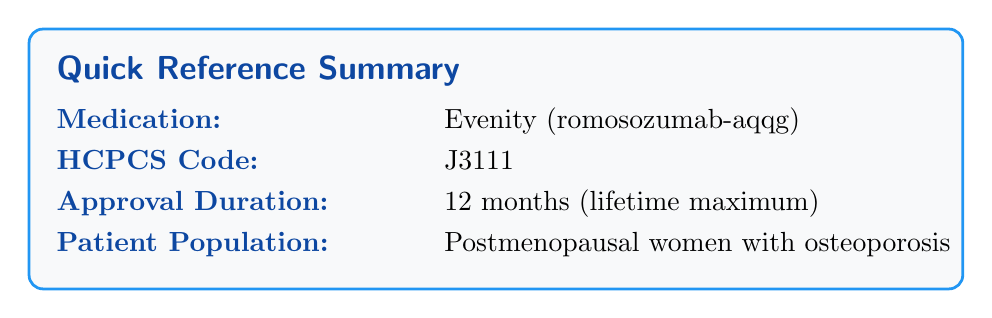
\begin{tikzpicture}
    \node[fill=lightgray, draw=accentblue, line width=1pt, rounded corners=5pt, inner sep=10pt] {
        \begin{minipage}{0.92\textwidth}
            \textcolor{darkblue}{\large\bfseries\sffamily Quick Reference Summary}
            \vspace{0.2cm}

            \begin{tabular}{@{}p{4.5cm}p{10cm}@{}}
                \textcolor{darkblue}{\bfseries Medication:} & Evenity (romosozumab-aqqg) \\[0.1cm]
                \textcolor{darkblue}{\bfseries HCPCS Code:} & J3111 \\[0.1cm]
                \textcolor{darkblue}{\bfseries Approval Duration:} & 12 months (lifetime maximum) \\[0.1cm]
                \textcolor{darkblue}{\bfseries Patient Population:} & Postmenopausal women with osteoporosis \\
            \end{tabular}
        \end{minipage}
    };
\end{tikzpicture}

\vspace{0.5cm}

\sectionheader{Prior Authorization Checklist}

\subsectionheader{STEP 1: Patient Demographics \& Diagnosis}

\begin{itemize}
    \item[\checkbox] \textbf{Patient is postmenopausal woman}
    \item[\checkbox] \textbf{Documented diagnosis of osteoporosis}
\end{itemize}

\subsectionheader{STEP 2: Bone Density Assessment}

\noindent\textcolor{mediumgray}{\bfseries At least ONE of the following must be documented:}

\begin{itemize}
    \item[\checkbox] T-score below -2.5
    \item[\checkbox] Patient at high risk for bone fracture
\end{itemize}

\subsectionheader{STEP 3: Prior Treatment History}

\noindent\textcolor{mediumgray}{\bfseries At least ONE of the following pathways must be met:}

\vspace{0.25cm}

\noindent
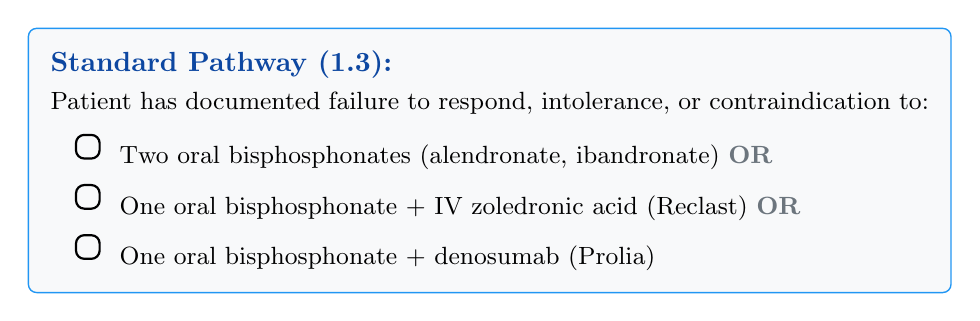
\begin{tikzpicture}
    \node[fill=lightgray, draw=accentblue, line width=0.5pt, rounded corners=3pt, inner sep=8pt] {
        \begin{minipage}{0.92\textwidth}
            \textcolor{darkblue}{\bfseries Standard Pathway (1.3):}\\[0.1cm]
            \small Patient has documented failure to respond, intolerance, or contraindication to:

            \begin{itemize}
                \item[\checkbox] Two oral bisphosphonates (alendronate, ibandronate) \textbf{\textcolor{mediumgray}{OR}}
                \item[\checkbox] One oral bisphosphonate + IV zoledronic acid (Reclast) \textbf{\textcolor{mediumgray}{OR}}
                \item[\checkbox] One oral bisphosphonate + denosumab (Prolia)
            \end{itemize}
        \end{minipage}
    };
\end{tikzpicture}

\vspace{0.2cm}

\noindent
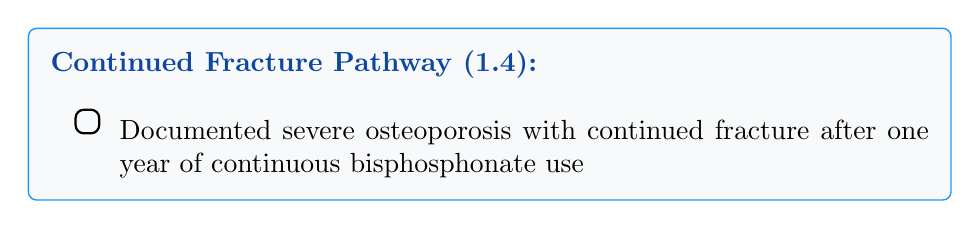
\begin{tikzpicture}
    \node[fill=lightgray, draw=accentblue, line width=0.5pt, rounded corners=3pt, inner sep=8pt] {
        \begin{minipage}{0.92\textwidth}
            \textcolor{darkblue}{\bfseries Continued Fracture Pathway (1.4):}

            \begin{itemize}
                \item[\checkbox] Documented severe osteoporosis with continued fracture after one year of continuous bisphosphonate use
            \end{itemize}
        \end{minipage}
    };
\end{tikzpicture}

\vspace{0.2cm}

\noindent
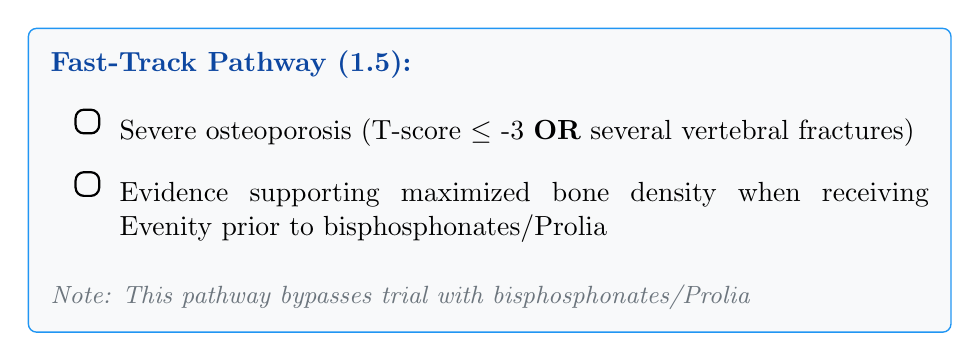
\begin{tikzpicture}
    \node[fill=lightgray, draw=accentblue, line width=0.5pt, rounded corners=3pt, inner sep=8pt] {
        \begin{minipage}{0.92\textwidth}
            \textcolor{darkblue}{\bfseries Fast-Track Pathway (1.5):}

            \begin{itemize}
                \item[\checkbox] Severe osteoporosis (T-score $\leq$ -3 \textbf{OR} several vertebral fractures)
                \item[\checkbox] Evidence supporting maximized bone density when receiving Evenity prior to bisphosphonates/Prolia
            \end{itemize}
            \vspace{0.1cm}
            \textcolor{mediumgray}{\small\textit{Note: This pathway bypasses trial with bisphosphonates/Prolia}}
        \end{minipage}
    };
\end{tikzpicture}

\subsectionheader{STEP 4: Exclusion Criteria Check}

\noindent\textcolor{warningred}{\bfseries All of the following must be confirmed as NO:}

\begin{itemize}
    \item[\checkbox] Patient is \textbf{NOT} using combination therapy (romosozumab with another bone mineral density modifying drug)
    \item[\checkbox] Patient does \textbf{NOT} have osteopenia (diagnosis must be osteoporosis)
    \item[\checkbox] Patient has \textbf{NOT} previously been treated with Forteo
    \item[\checkbox] Patient has \textbf{NOT} previously been treated with Tymlos
\end{itemize}

\vspace{0.4cm}

% Approval Decision Box
\noindent
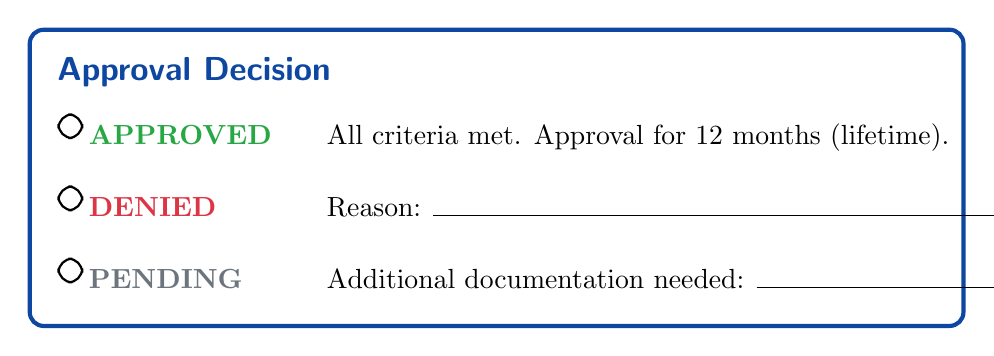
\begin{tikzpicture}
    \node[fill=white, draw=darkblue, line width=1.5pt, rounded corners=5pt, inner sep=10pt] {
        \begin{minipage}{0.92\textwidth}
            \textcolor{darkblue}{\large\bfseries\sffamily Approval Decision}
            \vspace{0.3cm}

            \begin{tabular}{@{}p{3cm}p{10.5cm}@{}}
                \checkbox \textcolor{successgreen}{\bfseries APPROVED} & All criteria met. Approval for 12 months (lifetime). \\[0.4cm]
                \checkbox \textcolor{warningred}{\bfseries DENIED} & Reason: \rule{7.5cm}{0.4pt} \\[0.4cm]
                \checkbox \textcolor{mediumgray}{\bfseries PENDING} & Additional documentation needed: \rule{5cm}{0.4pt} \\
            \end{tabular}
        \end{minipage}
    };
\end{tikzpicture}

\newpage

% Page 2 Header
\begin{tikzpicture}[remember picture,overlay]
    \fill[primaryblue] (current page.north west) rectangle ([yshift=-1.5cm]current page.north east);
\end{tikzpicture}

\vspace{0.3cm}

\begin{center}
    \textcolor{white}{\LARGE\bfseries\sffamily AI Usage Notes}
\end{center}

\vspace{0.5cm}

\sectionheader{How I Used the AI Tool}

I used \textbf{Claude} (Anthropic's AI assistant) throughout this assignment to transform the Health Alliance Policy \#2756P into a practical prior authorization checklist. Rather than simply asking the AI to ``do the work,'' I approached this as a collaborative problem-solving exercise where I directed the process and made key decisions about structure and design.

\sectionheader{My Process}

\textcolor{darkblue}{\bfseries\large Step 1: Read and Understand Everything First}\\[0.1cm]
I started by thoroughly reading both the Evenity policy PDF and the job description to understand:
\begin{itemize}
    \item What the policy actually requires for medication approval
    \item What Lamar Health does (automate complex medication paperwork)
    \item What the interviewer wants to see (communication skills, AI tool usage, practical problem-solving)
\end{itemize}

\vspace{0.25cm}

\textcolor{darkblue}{\bfseries\large Step 2: Consult with AI to Understand the Documents}\\[0.1cm]
I asked Claude to help me analyze what the policy documents were saying and identify the approval logic. My prompts included:
\begin{itemize}
    \item ``Can you align this md document with the pdf?'' --- to ensure accuracy
    \item ``What do you think they want me to do?'' --- to understand the assignment requirements
    \item ``What does a checklist for this project look like?'' --- to explore format options
\end{itemize}

This consultation helped me understand the complex conditional logic (1.3 OR 1.4 OR 1.5) and how it should be structured for end users.

\vspace{0.25cm}

\textcolor{darkblue}{\bfseries\large Step 3: Determine What the Interviewer Would Want}\\[0.1cm]
Based on the job description, I identified that Lamar Health needs someone who can:
\begin{itemize}
    \item Work effectively with AI/LLM tools (this is core to their product)
    \item Transform complex healthcare documents into actionable workflows
    \item Think about automation and practical implementation
    \item Communicate clearly about technical decisions
\end{itemize}

I decided the deliverable should show both \textit{what} I created (the checklist) and \textit{how} I thought through the problem (this document).

\vspace{0.25cm}

\textcolor{darkblue}{\bfseries\large Step 4: Format into LaTeX PDF}\\[0.1cm]
I chose LaTeX over a Google Doc because:
\begin{itemize}
    \item It demonstrates technical capability and attention to detail
    \item The professional typography makes the checklist look production-ready
    \item It shows I can work with developer tools, not just consumer apps
\end{itemize}

I asked Claude to generate the LaTeX code with specific design requirements: clean layout, checkboxes, visual hierarchy, and color-coded sections.

\vspace{0.25cm}

\textcolor{darkblue}{\bfseries\large Step 5: Review Contents Against Original Document}\\[0.1cm]
After the initial PDF was generated, I carefully verified that:
\begin{itemize}
    \item All approval criteria from the policy were accurately captured
    \item The logic matched the source document (not simplified or misinterpreted)
    \item No requirements were missed or added incorrectly
    \item Medical terminology and drug names were spelled correctly
\end{itemize}

\vspace{0.25cm}

\textcolor{darkblue}{\bfseries\large Step 6: Iterate on Design}\\[0.1cm]
I asked Claude to ``make it beautiful'' and iterated on the visual design:
\begin{itemize}
    \item Added color coding (blue headers, boxed pathways, color-coded decisions)
    \item Used rounded corners and modern styling for a professional look
    \item Organized content into clear steps that mirror the decision flow
    \item Ensured the design was functional, not just decorative
\end{itemize}

The goal was to create something that looks like a real product, not just an assignment.

\newpage

% Page 3 Header
\begin{tikzpicture}[remember picture,overlay]
    \fill[primaryblue] (current page.north west) rectangle ([yshift=-1.5cm]current page.north east);
\end{tikzpicture}

\vspace{0.3cm}

\begin{center}
    \textcolor{white}{\LARGE\bfseries\sffamily Challenges \& Solutions}
\end{center}

\vspace{0.5cm}

\sectionheader{Challenges Encountered}

\textcolor{darkblue}{\bfseries\large Challenge 1: Understanding Policy Logic}\\[0.1cm]
The original policy had complex conditional logic (1.3 OR 1.4 OR 1.5), with 1.3 itself containing three OR conditions. I worked with Claude to clarify this by creating three distinct ``pathways'' rather than a confusing nested checklist.

\vspace{0.25cm}

\textcolor{darkblue}{\bfseries\large Challenge 2: Ambiguity in Criterion 1.3}\\[0.1cm]
The policy states ``Documented failure to respond, intolerance, or contraindication to any of the following: OR'' followed by three bullet points. It was unclear whether patients needed to fail ALL options or just ONE. Based on the policy language and standard medical practice, I interpreted this as needing to fail at least ONE of the three combinations, which Claude helped clarify and structure.

\vspace{0.25cm}

\textcolor{darkblue}{\bfseries\large Challenge 3: Balancing Completeness with Usability}\\[0.1cm]
The policy contains extensive references and disclaimers that are important for legal purposes but would clutter an operational checklist. I focused on extracting only the actionable approval criteria while maintaining accuracy to the source policy.

\vspace{0.25cm}

\textcolor{darkblue}{\bfseries\large Challenge 4: Making it Practical}\\[0.1cm]
Healthcare workers need to make quick decisions. I collaborated with Claude to organize the checklist into a step-by-step flow that mirrors the actual decision-making process, rather than just copying the policy's original structure.

\vspace{0.4cm}

\sectionheader{Why This Approach Works}

This checklist transforms a 2-page legal policy document into a tool that can be:

\begin{itemize}
    \item \textcolor{darkblue}{\bfseries Used by pharmacy technicians or nurses} without deep policy knowledge
    \item \textcolor{darkblue}{\bfseries Automated using AI/LLM technology} (like what Lamar Health builds)
    \item \textcolor{darkblue}{\bfseries Integrated into electronic health record (EHR) systems}
    \item \textcolor{darkblue}{\bfseries Updated quickly} when policy requirements change
\end{itemize}

\vspace{0.2cm}

\noindent
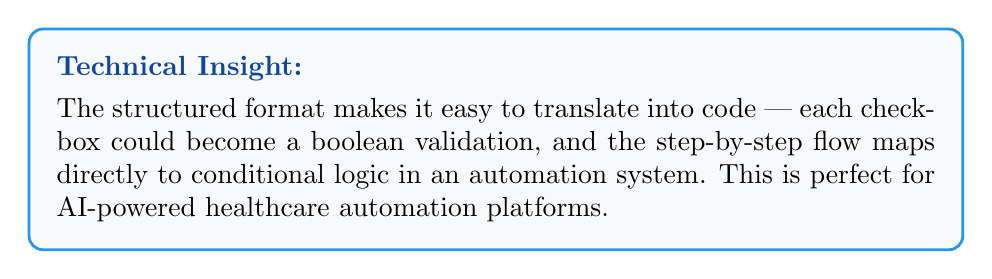
\begin{tikzpicture}
    \node[fill=lightgray, draw=accentblue, line width=1pt, rounded corners=5pt, inner sep=10pt] {
        \begin{minipage}{0.92\textwidth}
            \textcolor{darkblue}{\bfseries Technical Insight:}\\[0.1cm]
            The structured format makes it easy to translate into code --- each checkbox could become a boolean validation, and the step-by-step flow maps directly to conditional logic in an automation system. This is perfect for AI-powered healthcare automation platforms.
        \end{minipage}
    };
\end{tikzpicture}

\vspace{0.6cm}

\begin{center}
    
\begin{tikzpicture}
        \draw[line width=1pt, darkblue] (0,0) -- (12,0);
    \end{tikzpicture}

    \vspace{0.3cm}

    \textcolor{darkblue}{\bfseries Document prepared by:} [Your Name]\\
    \textcolor{mediumgray}{\bfseries Date:} \today\\
    \textcolor{mediumgray}{\bfseries Contact:} [Your Email]
\end{center}

\end{document}